\documentclass{beamer}
\usepackage{graphicx}
\usepackage{amsmath}
\DeclareMathOperator{\tr}{tr}

\usetheme{default}

\title[JC: QM Closure for PDEs]{Quantum mechanical closure of partial differential equations with symmetries}
\author{Chris Vales, David C. Freeman, Joanna Slawinska, Dimitrios Giannakis}
\institute{Department of Mathematics, Dartmouth College}
\date{Journal Club Presentation}

\begin{document}

\begin{frame}
    \titlepage
    \begin{center}
        \vspace{1cm}
        Presented by: [Your Name]
    \end{center}
\end{frame}

\begin{frame}{Motivation: The Closure Problem}
    \begin{itemize}
        \item Complex dynamical systems (e.g., climate, turbulence) have degrees of freedom evolving across a wide range of spatial and temporal scales.
        \item It's often computationally impossible to simulate all scales directly.
        \item We separate the system into:
        \begin{itemize}
            \item \textbf{Resolved} (coarse-grain) degrees of freedom that we can simulate.
            \item \textbf{Unresolved} (fine-grain) degrees of freedom that are too expensive.
        \end{itemize}
        \item \textbf{The Closure Problem:} How can we approximate the effects (fluxes) of the unresolved dynamics on the resolved dynamics?
        \item \textbf{Goal:} Build a surrogate model for these unresolved fluxes.
    \end{itemize}
\end{frame}

\begin{frame}{Challenges \& This Paper's Approach}
    \begin{itemize}
        \item \textbf{Deterministic Models:} Modeling unresolved variables as a simple function of resolved ones reduces the state-space dimension.
        \begin{itemize}
            \item This can lead to a loss of complex or chaotic behavior, making the model less accurate.
        \end{itemize}
        \vspace{0.5cm}
        \item \textbf{Stochastic Models:} A common alternative that introduces a surrogate state space for the unresolved variables to maintain complexity.
        \vspace{0.5cm}
        \item \textbf{This Paper's Approach:} A framework called \textbf{Quantum Mechanical Closure (QMCl)} that generalizes stochastic modeling.
        \begin{itemize}
            \item It models the unresolved degrees of freedom as a quantum mechanical system.
        \end{itemize}
    \end{itemize}
\end{frame}

\begin{frame}{Core Idea: Quantum Mechanical Closure (QMCl)}
    \begin{itemize}
        \item The classical dynamics are embedded into an infinite-dimensional quantum mechanical system.
        \item \textbf{Unresolved State:} Represented by a quantum density operator ($\rho$).
        \item \textbf{Unresolved Fluxes:} Calculated as expectation values of quantum observables ($A_j$).
        \[ \tilde{z}_j(\rho) = \tr(\rho A_j) \]
        \item \textbf{Dynamics of the Quantum State:}
        \begin{itemize}
            \item \textbf{Prediction:} The quantum state is evolved forward in time using a transfer operator ($\mathcal{P}^L$).
            \item \textbf{Correction:} The state is updated (conditioned) based on new observations of the resolved state via a quantum analogue of Bayes' rule.
        \end{itemize}
        \item A key benefit is automatic \textbf{positivity preservation}, crucial for physical quantities like density or temperature.
    \end{itemize}
\end{frame}

\begin{frame}{Main Contribution: Extending QMCl to PDEs}
    This work extends the QMCl framework from ODEs to spatiotemporal dynamics governed by PDEs.
    \vspace{0.5cm}
    \textbf{Key Features of the Extended Framework:}
    \begin{enumerate}
        \item \textbf{Positivity Preservation:} Inherited from the original QMCl, ensuring physically meaningful flux estimates.
        \vspace{0.2cm}
        \item \textbf{Symmetry Factorization:} Intelligently handles spatial symmetries (like translation) to create a highly compressed and efficient representation of the dynamics.
        \vspace{0.2cm}
        \item \textbf{Computational Efficiency:} Employs modern numerical methods (low-rank matrix approximations) to make the data-driven approach tractable for large systems.
        \vspace{0.2cm}
        \item \textbf{Application:} Successfully applied to a challenging closure problem for the shallow water equations.
    \end{enumerate}
\end{frame}

\begin{frame}{Method: Handling Symmetries with Kernels}
    The framework combines QMCl with \textbf{Vector Valued Spectral Analysis (VSA)}.
    \begin{itemize}
        \item A kernel function is used to measure similarity between spatiotemporal data points $(x, s)$.
        \item \textbf{Delay Embedding:} To capture dynamics, the kernel compares not just single states, but short, spatially-local time series (delay coordinates).
        \[ W_Q((x,s)) = (\hat{x}(s), \hat{x}(\Phi^{-\Delta t}(x))(s), \dots) \]
        \item \textbf{Symmetry Invariance:} The eigenfunctions derived from this kernel are constructed to be \textbf{invariant} under the system's spatial symmetries.
        \item This avoids redundant "copies" of patterns, leading to a very efficient basis for representing the spatiotemporal dynamics.
    \end{itemize}
\end{frame}

\begin{frame}{Application: Shallow Water Equations}
    \begin{itemize}
        \item A standard testbed for fluid dynamics, modeling the evolution of fluid height ($h$) and momentum ($q$).
        \item \textbf{The Closure Problem Setup:}
        \begin{itemize}
            \item A "true" high-resolution simulation is run on a \textbf{fine grid} (1920 cells).
            \item The \textbf{resolved state} ($\hat{x}$) is created by averaging the true state onto a \textbf{coarse grid} (96 cells).
            \item The \textbf{unresolved fluxes} ($G_m$) are the correction terms needed to make the coarse simulation accurate.
        \end{itemize}
        \item \textbf{Goal:} Train a QMCl model to predict the subgrid fluxes ($G_m$) using only the coarse-grid state ($\hat{x}_m$).
    \end{itemize}
\end{frame}

\begin{frame}{Training and Basis Functions}
    \begin{itemize}
        \item The model is trained on data from 3 different initial conditions.
        \item The kernel method generates a set of spatiotemporal basis functions ($\phi_\ell$) that are optimized to represent the system's dynamics.
    \end{itemize}
    \begin{figure}
        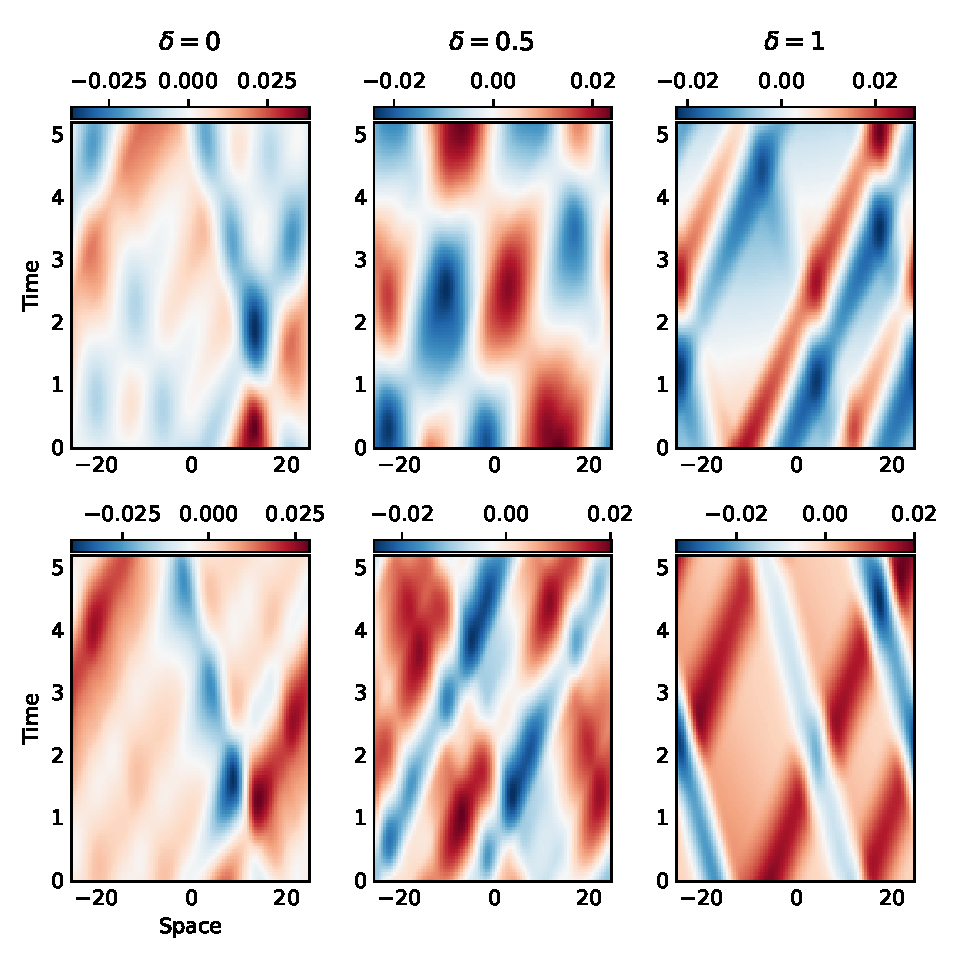
\includegraphics[width=0.8\textwidth]{paper/vsabasis.pdf}
        \caption{Examples of the learned basis functions. They capture the essential dynamics (propagating wave fronts) and are invariant to spatial translation, making them very efficient.}
        \label{fig:vsa-basis}
    \end{figure}
\end{frame}

\begin{frame}{Results: Out-of-Sample Prediction}
    The trained model was tested on a new initial condition it had \textbf{not} seen during training.
    \begin{figure}
        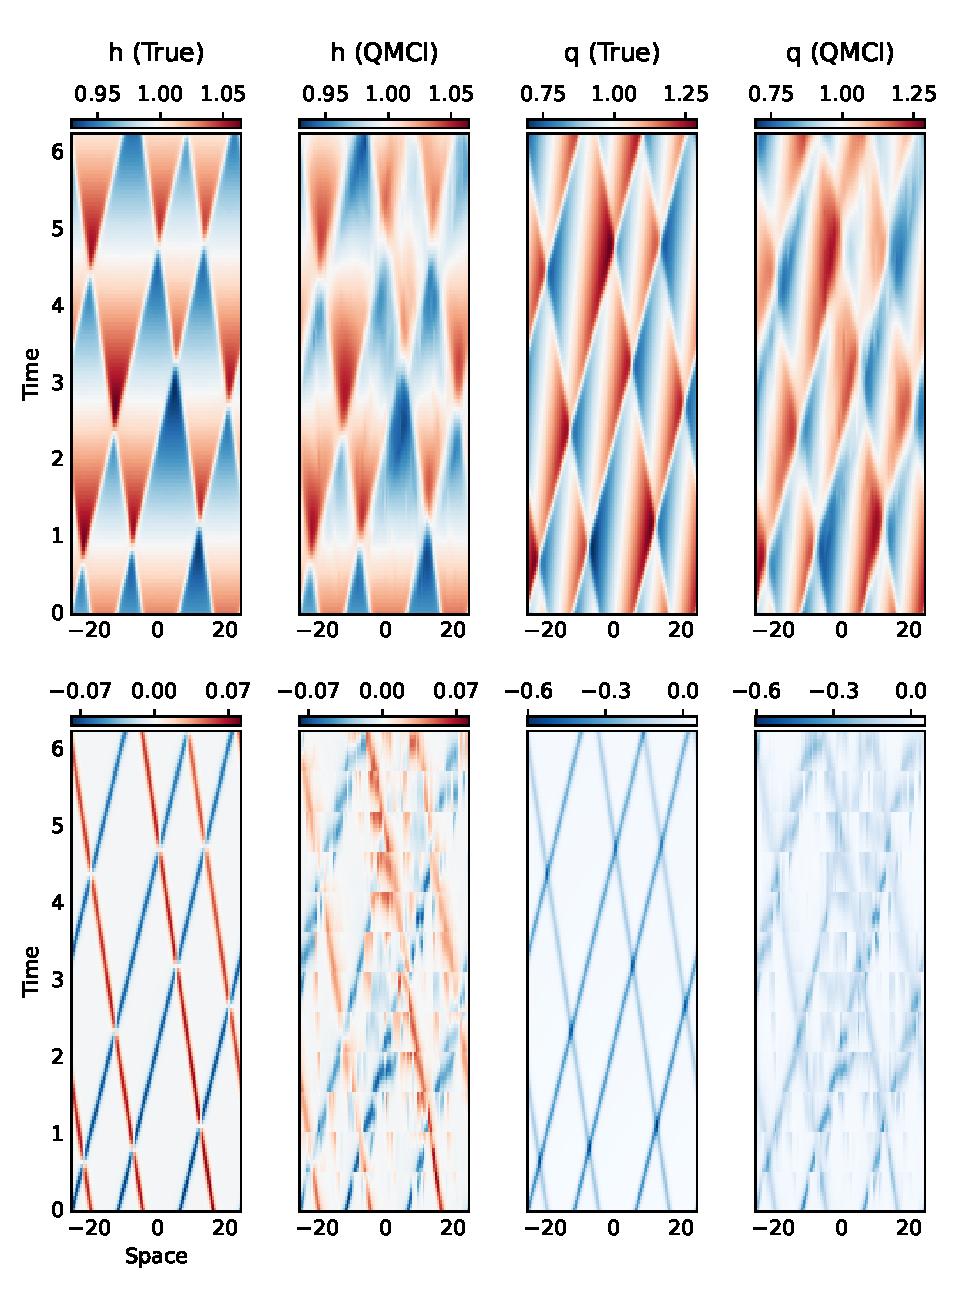
\includegraphics[width=0.9\textwidth]{paper/res01a.pdf}
        \caption{Prediction for an out-of-sample trajectory. Top: Resolved state ($h, q$). Bottom: Subgrid fluxes. (Left: True, Right: QMCl Prediction).}
        \label{fig:res01a}
    \end{figure}
    \textbf{Observation:} The QMCl model accurately captures the main features of both the resolved state and the unresolved fluxes.
\end{frame}

\begin{frame}{Conclusion}
    \begin{itemize}
        \item This paper presents a successful extension of the QMCl framework to PDEs, which is a significant step towards real-world applications.
        \vspace{0.5cm}
        \item The combination of QMCl with VSA provides a powerful, data-driven method that respects physical constraints (positivity) and efficiently handles symmetries.
        \vspace{0.5cm}
        \item The model demonstrated strong predictive performance on a challenging closure problem for the shallow water equations, even for out-of-sample initial conditions.
    \end{itemize}
\end{frame}

\end{document}
